\documentclass[conference]{IEEEtran}

% *** GRAPHICS RELATED PACKAGES ***
%
\ifCLASSINFOpdf
  % \usepackage[pdftex]{graphicx}
  % declare the path(s) where your graphic files are
  % \graphicspath{{../pdf/}{../jpeg/}}
  % and their extensions so you won't have to specify these with
  % every instance of \includegraphics
  % \DeclareGraphicsExtensions{.pdf,.jpeg,.png}
\else
  % or other class option (dvipsone, dvipdf, if not using dvips). graphicx
  % will default to the driver specified in the system graphics.cfg if no
  % driver is specified.
  % \usepackage[dvips]{graphicx}
  % declare the path(s) where your graphic files are
  % \graphicspath{{../eps/}}
  % and their extensions so you won't have to specify these with
  % every instance of \includegraphics
  % \DeclareGraphicsExtensions{.eps}
\fi
% graphicx was written by David Carlisle and Sebastian Rahtz. It is
% required if you want graphics, photos, etc. graphicx.sty is already
% installed on most LaTeX systems. The latest version and documentation
% can be obtained at: 
% http://www.ctan.org/pkg/graphicx
% Another good source of documentation is "Using Imported Graphics in
% LaTeX2e" by Keith Reckdahl which can be found at:
% http://www.ctan.org/pkg/epslatex
%
% latex, and pdflatex in dvi mode, support graphics in encapsulated
% postscript (.eps) format. pdflatex in pdf mode supports graphics
% in .pdf, .jpeg, .png and .mps (metapost) formats. Users should ensure
% that all non-photo figures use a vector format (.eps, .pdf, .mps) and
% not a bitmapped formats (.jpeg, .png). The IEEE frowns on bitmapped formats
% which can result in "jaggedy"/blurry rendering of lines and letters as
% well as large increases in file sizes.
%
% You can find documentation about the pdfTeX application at:
% http://www.tug.org/applications/pdftex

\usepackage{xcolor}

\usepackage{graphicx}
\usepackage{enumitem}
\usepackage{amsmath,amsthm,amsfonts}
\usepackage{hyperref}

\usepackage{listings}
\definecolor{mGreen}{rgb}{0,0.6,0}
\definecolor{mGray}{rgb}{0.5,0.5,0.5}
\definecolor{mPurple}{rgb}{0.58,0,0.82}
\definecolor{backgroundColour}{rgb}{0.95,0.95,0.92}
\lstdefinestyle{CStyle}{
    backgroundcolor=\color{backgroundColour},   
    commentstyle=\color{mGreen},
    keywordstyle=\color{magenta},
    numberstyle=\tiny\color{mGray},
    stringstyle=\color{mPurple},
    basicstyle=\footnotesize,
    breakatwhitespace=false,         
    breaklines=true,                 
    captionpos=b,                    
    keepspaces=true,                 
    numbers=left,                    
    numbersep=5pt,                  
    showspaces=false,                
    showstringspaces=false,
    showtabs=false,                  
    tabsize=2,
    language=C
}
\usepackage[numbers, comma, square]{natbib}
\bibliographystyle{unsrtnat}
\usepackage{url}
%\usepackage[backend=biber,style=numeric,sorting=none]{biblatex}
%\addbibresource{sample.bib}

% correct bad hyphenation here
\hyphenation{op-tical net-works semi-conduc-tor}


\begin{document}
\title{Hardware Security \\ Meltdown and Spectre Attacks}


% author names and affiliations
% use a multiple column layout for up to three different
% affiliations
\author{
    \IEEEauthorblockN{David Rainho}
    \IEEEauthorblockA{up201906994@up.pt}
    \and
    \IEEEauthorblockN{Gabriel Oliveira}
    \IEEEauthorblockA{up201904824@up.pt}
    \and
    \IEEEauthorblockN{Jorge Pais}
    \IEEEauthorblockA{up201904841@up.pt}
    \and
    \IEEEauthorblockN{Tiago Sousa}
    \IEEEauthorblockA{up201907205@up.pt}
}


% make the title area
\maketitle

% As a general rule, do not put math, special symbols or citations
% in the abstract
\begin{abstract}
This paper aims to provide a comprehensive overview of the Meltdown and Spectre attacks, which attempt to read privileged memory space by exploiting faults in some microprocessor architectures. As to practice the concepts studied, some results and the main conclusions from the SEED Labs are presented. Furthermore, a practical application of the Spectre exploit was developed in order to both demonstrate how a real-world attack could be performed to steal data from a vulnerable Kernel module. Finally, some information about the currently available mitigation strategies for these attacks are presented.

\end{abstract}

\section{Introduction}
Meltdown and Spectre attacks were disclosed in 2018 and exploited existing vulnerabilities on modern processor architectures, such as those from the likes of Intel, ARM, and AMD. These attacks aim to break the memory isolation barriers between user processes and the kernel.

Both attacks make use of faults in CPU speculative execution subsystems, that combined with a cache side-channel attack, enable a rouge user to gain access to privileged data, otherwise inaccessible. Despite these fundamental similarities, they are also different in many other aspects. Whilst Meltdown exploits out-of-order execution to gain illegal access to kernel memory, Spectre attacks use branch prediction techniques to trick other programs into leaking their own private memory. Although some patches and mitigation strategies have been made available after the disclosure of these attacks, they can still be implemented in some systems.

\section{Theoretical background}

In this section, we describe some theoretical aspects behind this kind of attack, as well as a brief description of both the Meltdown and Spectre vulnerabilities.

\subsection{Speculative execution}
One of the major breakthroughs in terms of performance during the evolution of the CPU was the introduction of pipelined processor architectures in which several instructions could be concurrently fetched, decoded and executed, maximizing CPU usage per clock cycle \cite{bookPatterson}.

However, some instructions are dependent on others, for instance, reading a variable from memory whose value is needed to execute an addition operation, being that the read instruction is much slower than the addiction. This dependence in some cases may lead to the need of stalling the CPU and thus reducing its efficiency. To further increase CPU performance, engineers started to employ speculative execution techniques that aim to minimize the impact of the dependencies between instructions. This approach consists in executing instructions ahead of their time (for a normal pipelined architecture) most of the time assuming the validity of previous instructions without knowing all the necessary conditions to evaluate them, resulting in a performance gain if the guessed conditions are correct. Some examples of applications of this technique are:
\begin{itemize}
  \item \textbf{Branch prediction} - executing instructions ahead of their time that are dependent on a branch condition for which the CPU tries to make educated guesses about - used in Spectre;
  \item \textbf{Out-of-order execution} - rearranging the order in which the instructions are executed so that slower instructions, such as reading from memory, are run ahead of their time in order that they are already available when needed, minimizing CPU idle time - used in Meltdown.
  % Processing instructions ahead of their time, ignoring the order that the program has so that while a slow instruction is being processed a faster one can be dealt with. Even when these instructions depend on each other for validation purposes, an instruction that comes later in the program can be executed before an earlier instruction. This tactic minimizes the CPU's downtime as slower instructions can be done in parallel with their following counter-parts.
\end{itemize} 

%Nowadays, most CPUs apply these techniques as they offer considerable performance gains. However, they can also be used to execute attacks capable of leaking sensitive information that shouldn't be accessed by user-level applications, as we shall demonstrate on this paper.

\subsection{Memory access times}

One of these attacks' basis is the time that the CPU takes to access a stored value. The minimization of these access times is critical for CPU efficiency so, in modern computers, in order to improve  access time to values in memory and avoid increasing technology costs, the solution found was introducing a hierarchy of smaller, but faster memories between the processor and main memory, known as caches. Their introduction creates a clearly distinct time behavior for when a CPU loads a stored value: accessing the main memory may take hundreds of more clock cycles than loading a value stored on the cache as can be seen in Figure \ref{fig:memAccess}.
\begin{figure}[h]
  \centering
  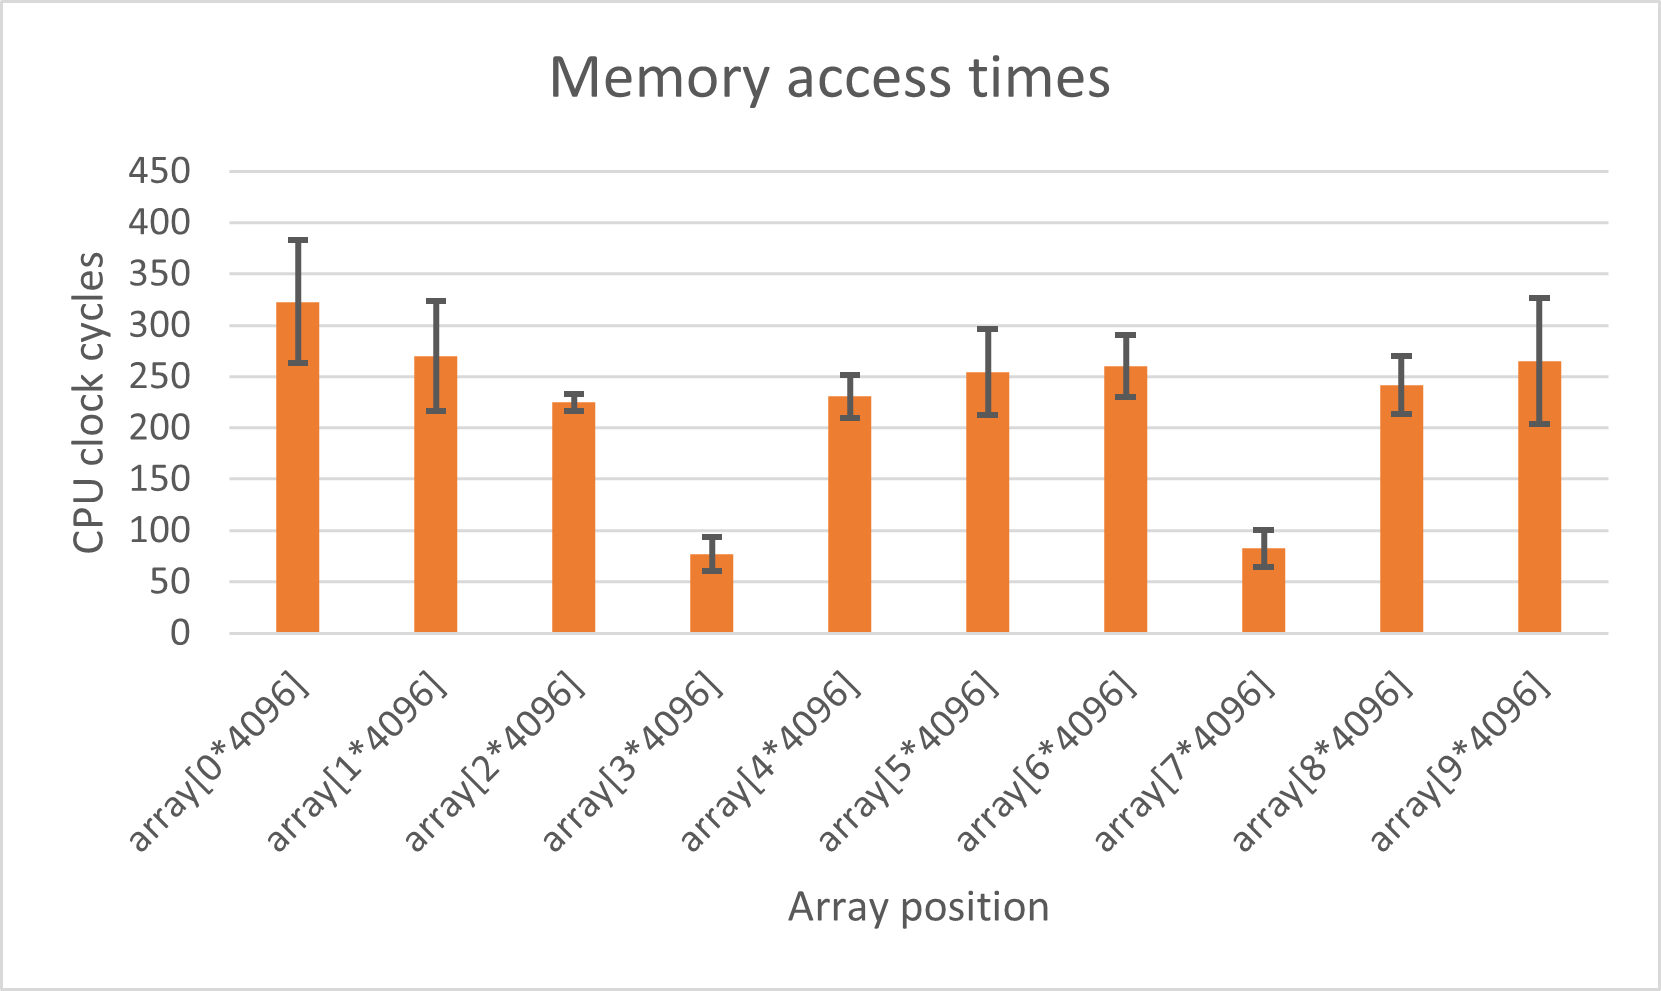
\includegraphics[width=0.4\textwidth]{figures/Memory_Access.png}
  \caption{Memory Access Times}
  \label{fig:memAccess}
\end{figure}
It shows the measured mean access times and the 95\% confidence interval of ten tries for an array with ten positions. Positions three and seven were previously loaded into the cache while the rest are on the main memory. It is clear that based on the measured access times it is possible to infer whether or not a value was on the cache or on that main memory, which provides a way to retrieve secret values as will be explained in the next sections.



\subsection{Side channel attacks - FLUSH+RELOAD}
The use of speculative execution techniques can indeed be used by an attacker program to gain access to information that, in normal circumstances should not be accessible. Nevertheless, the attacker still can't directly access that stolen information as it has no permission to do that. So, in order to fully leak the private data stolen, the attacker needs to create some sort of side channel. A side channel attack is a means to extract private information from some system without accessing it directly, it exploits observable side effects such as timing behavior or power consumption to gain access to private information.
\par There are various types of side-channel attacks. One of the most common is FLUSH+RELOAD \cite{flushReload}, which is what's usually employed on Meltdown and Spectre attacks. This attack relies on the different temporal behavior of accessing the memory content stored in the cache and on the main memory, which is faster and slower, respectively. In a simplistic way, the FLUSH+RELOAD may be divided into the following three steps:
\begin{enumerate}
    \item \textbf{FLUSH} - Clean, i.e., remove contents, of a defined number of cache positions, for instance, all cache locations where a 256 positions array is stored;
    \item \textbf{Attack} - Let the attack proceed, expecting that the stolen secret is used to read some memory data so that the data corresponding to that address is stored on the cache;
    \item \textbf{RELOAD} - Read all array positions, measuring the time it takes to reload each element. If one is faster than the other, the attacker can be mostly sure that it was stored in the cache and can infer what the memory position accessed with the victim's data.
\end{enumerate}
There are some other considerations that should be taken into account and handled accordingly when performing this kind of attack, such as the concepts of spatial locality that may make the cache load contiguous memory pages and some countermeasures for cache side-channel attacks that might be implemented.


\section{Attack's description and implementation}
\par This section introduces the Meltdown and Spectre and demonstrates how a simple version of those attacks could be implemented. Most of the work here described is based on the implementations described in the studied SEED labs.

\subsection{Meltdown attack}
The original Meltdown attack (\href{https://nvd.nist.gov/vuln/detail/CVE-2017-5754}{CVE-2017-5754}) aims to break the isolation between the kernel and user-level processes and can, theoretically, be used to leak all kernel data \cite{meltdownPaper}. In order to do so, it tries to exploit a vulnerability in the out-of-order execution engine of some CPU architectures. When a user-level program tries to access unauthorized memory the security permissions checks must fail and an exception should be raised. For instance, in the code presented on the following listing, the second line should never be executed, since the program has no permission to access that data.
\begin{lstlisting}[style=CStyle, caption=Accessing kernel memory , label=code_snippet2]
kernel_data = *kernel_address;
number = number + kernel_data;
\end{lstlisting}
\par However, when an instruction is executed out-of-order, that permissions verification cannot occur beforehand, as that would defeat the purpose of executing out-of-order. In fact, there's a race condition between the arrival of the kernel data and the permission check results which may allow it to execute the second line. By giving the CPU some extra work as done in the following listing, the time window between the arrival of the data and the permissions verification can be extended, thus increasing the success rate of the attack.
\begin{lstlisting}[style=CStyle, caption=Assembly code that increases success rate , label=code_snippet2]
asm volatile(
   ".rept 400;"                
   "add $0x141, %%eax;"
   ".endr;"                    
   : "eax"
); 
\end{lstlisting}
\par Nevertheless, the permission check results will arrive, an exception will be raised, the program stopped and the secret cannot be retrieved. In a safe CPU, all data related to those instructions should be dumped upon the exception triggering, so that no information can be extracted. Nevertheless, some vulnerable CPU architectures, don't proceed that way, since they leave noticeable effects on the cache, even after the exception is raised. So the next step in the implementation of Meltdown is handling the raised exception. There are several ways of doing this, such as the use of forks so that the invalid memory access is done on the child program but, for our implementation, we've opted for the \texttt{sigsetjmp()}, \texttt{siglongjmp()}, that emulate, in C, the behavior of a try/catch exception handling method.
\par With the kernel memory leaked and the exception handling, the only thing left is making the stolen data available to the attacker. For that, we've used a cache side-channel attack: FLUSH+RELOAD. As already explained, this attack requires first the flush from the cache of the memory addresses of an array. Then, replace the second line of Listing 1 by
\begin{lstlisting}[style=CStyle, caption=Retrieving the data , label=code_snippet3]
array[kernel_data * 4096 + DELTA] += 1;   
\end{lstlisting}
we can mostly be sure that that position was loaded into the cache. Lastly, by loading all array positions (256, in this case, to form a byte) and measuring access times, we can infer what the kernel data was. By changing the address of kernel data, we can leak the full secret and, in the limit, all kernel memory.
\par Although sometimes successful, this method is not fully reliable, as the error rates are relatively large. There are many improvements to increase the accuracy of this attack. One of the simplest is employing a statistical method, in which all memory addresses are accessed multiple times, accepting as correct the leaked value that got the maximum number of hits. Using this technique the accuracy on our tests skyrocketed, to 49 hits on 50 tries which indicates an accuracy of 98\%.
\par In this section the Meltdown attack was described and a possible simple implementation was demonstrated. Nevertheless, it is important to state that in our implementation we've loaded the secret into the kernel, therefore we knew beforehand its address, thus we can make sure that it will be loaded to the cache when necessary. This is a major simplification from a real-world attack, that would need an extra step to determine the address of the memory of interest.




\subsection{Spectre attack}
This method exploits the speculative execution of code during direct (\href{https://nvd.nist.gov/vuln/detail/CVE-2017-5753}{CVE-2017-5753}) or indirect (\href{https://nvd.nist.gov/vuln/detail/CVE-2017-5715}{CVE-2017-5715}) branching. In a processor, branching completion can be slow, mostly due to the time required to evaluate conditions that involve loading values from memory. So as to increase performance, modern CPUs implement branch prediction and attempt to anticipate, based on previous branches, which sequence of instructions to run speculatively. After checking the validity of the condition, if it is correct, the processor continues the nominal program execution, otherwise, the processor discards the results of the instructions. Although the CPU reverts to a nominal state, values that were cached during its execution remain cached. Also, because branch prediction usually accounts for past branches, it is possible for an attacker to influence the decision taken.

\subsubsection{Variant 1 - Direct branching (bypass out-of-bounds check)}
As for the original paper, we will explain how the vulnerability can be exploited for the particular case of a conditional branch. The following code will bridge the example given in \cite{spectrePaper}, the Spectre SEED Lab, and the developed proof-of-concept.

The code snippet in Listing \ref{code_snippet} may appear within functions (such as kernel syscalls). This one receives an unsigned x value from an untrusted source.
\begin{lstlisting}[style=CStyle, caption=Conditional branching, label=code_snippet]
if (x < array1_size)
    y = array2[array1[x]*4096];
\end{lstlisting}
The process running the code has an array named \texttt{array1} with fixed length \texttt{array1\_size} (for SEED Labs, it corresponds to the \texttt{buffer} array of integer values and type \texttt{uint8\_t}). The values of \texttt{array1[x]} will be given in the interval 0 to 255, so the size of \texttt{array2} is $256*4096$ bytes long. The constant value 4096 is greater than the block/line size of the L1 cache and guarantees that two adjacent array1 values do not end up cached simultaneously (they aren't near each other in memory).

Starting the analysis, we assume \texttt{array1\_size} and \texttt{array2} are not cached, which is possible to do in our custom C program with \texttt{\_mm\_clflush} (for every position of \texttt{array2}) or forcing it by caching other values from memory (Evict). The misprediction and its exploitation will work as follows:
\begin{enumerate}
    \item \textbf{Training}, start by performing a set of true conditions, biasing the decision-making to be true for the next evaluation;
    \item \textbf{Out--of--bound check}, use an invalid value for x (i.e. $\Tilde{x} >$ \texttt{array1\_size}). The verification will be slow because \texttt{array1\_size} has to be cached and then compared;
    \item \textbf{Speculative execution}, while the condition isn't checked, the processor will assume a true condition and gets the out-of-bounds \texttt{array1[$\Tilde{x}$]} (cache hit). Then, the value \texttt{array2[array1[$\Tilde{x}$]*4096]} will be cached after a miss;
    \item \textbf{Side-channel}, if the procedure was successful until this step, one and only one position/value of \texttt{array2} (from the 256 possible) is now in Cache. Notice, the information of 8 bytes (256 bits) in \texttt{k=array1[$\Tilde{x}$]} sets the only position cached \texttt{array2[k]};
    \item \textbf{Retrieved information}, if the attacker has access to \texttt{array2}, it can retrieve the 256 different values while measuring the time required to obtain them. Remember that cached values are faster to access, so \texttt{array2[i]} will be faster for i=k, than for i!=k. This way, we know the position k, which in turn means we know the byte in address \texttt{$array1[\Tilde{x}]$}.
\end{enumerate}

This attack may fail in each step, due to ill training, values aren't properly flushed out or the time required to get \texttt{array2[array1[x]*4096]} is greater than the time to evaluate the condition.

\subsubsection{Variant 2 - Indirect branching (branch target injection)}
In a similar manner to the first variant, the computer where a program is running tries to speculatively run instructions, but now this is based on the prediction of an address, instead of a condition. An attacker has the objective of deceiving the processor into executing instructions that leak information (gadgets). Gadgets are sequences of instructions that should be relatively simple, so as to run while the processor doesn't retrieve a nominal execution. After locating an indirect branch, it could be exploited at a high level as follows:
\begin{enumerate}
    \item \textbf{Training}, change the address for the next prediction to be that of the gadget by, for example accessing the branch target buffer and inserting the respective offset to the gadget address;
    \item \textbf{Gadget}, may leak data to a side--channel by performing cache-timing, similarly to variant 1;
\end{enumerate}

While this attack poisons the branch target buffer, it can be done to the Return Stack Buffer (RSB) or Branch History Buffer (BHB). Also, it may be worth noting that the prediction method may change between processors. This also applies to different generations of the same CPU.

\section{Contribution}

For the final part of this work, a simple proof-of-concept was developed to demonstrate how a Spectre-styled attack could be used to leak kernel memory and for that matter, memory from other processes. In order to do so, a very simple device driver was implemented which exposed a \textit{/proc/} file using Linux's \textit{seq\_file} interface \cite{seqFile}. Using this device driver, a secret string is placed within the kernel memory like with the Meltdown SEED labs attack. Essentially, the \textit{/proc/} file when read returns the memory address of the first byte within this secret string, and as such the objective is to read this value from user space. During this read, it is made sure that the values of the secret string are stored in the cache, so as to guarantee that the Branch Prediction Unit speculates upon the result of the array-bound condition and that the program does not have to wait for this value to be read from memory.  

From the attacking program point of view, the structure of the attack is very similar to that of the one used during the SEED Labs. A simple depiction of the attack structure can be seen in Figure \ref{fig:spectreFlowchart}. The program works by attempting to access kernel memory speculatively through accesses to a local array named \texttt{buffer}. The code presented below in listing \ref{specExec} shows the function where speculative execution happens.

\begin{lstlisting}[style=CStyle, caption=speculativeExec() function, label=specExec]
void speculativeExec(size_t a){
    _mm_clflush(&size_buffer);
    for(int i = 0; i < 256; ++i)
        _mm_clflush(&array[4096*i + 1024]);

    if(a < size_buffer)
        array[buffer[a] * 4096 + 1024] += 1;
}
\end{lstlisting}

This code is then used to both mistrain the BPU and attempt to access kernel memory, leaving traces of the results in the cache. As before, FLUSH + RELOAD is used to extract these values from the CPU. The attack is run multiple times for each character in order to obtain a statistically stronger result for each value, and then this loop is run for several address offsets in order to obtain all the bytes contained in the secret string.

\begin{figure}[h]
    \centering
    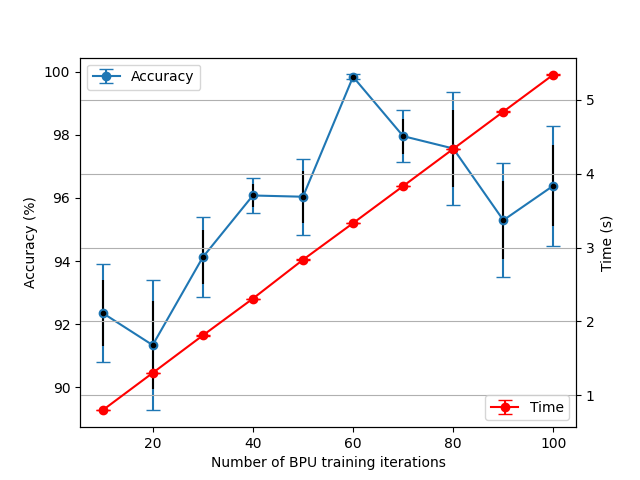
\includegraphics[width=0.5\textwidth]{figures/resultsAccuracyTime.png}
    \caption{Accuracy and execution time results}
    \label{fig:accuracyResults}
\end{figure}

After developing the code, it was noticed that by having the same number of BPU mistraining iterations as the SEED Labs, which were 1000, the attack took quite a while to leak a 50 byte string. So in order to verify how much the attack accuracy depends on this step, the attack was run multiple times, and the accuracy and total run time were measured. These results can be found in Figure \ref{fig:accuracyResults}. From these, it was possible to verify that the attack is overall pretty successful, even with the lower number of iterations when compared to the SEED Labs, and that by using less BPU training iterations data can be leaked at a greater cadence.

\begin{figure}[h]
  \centering
  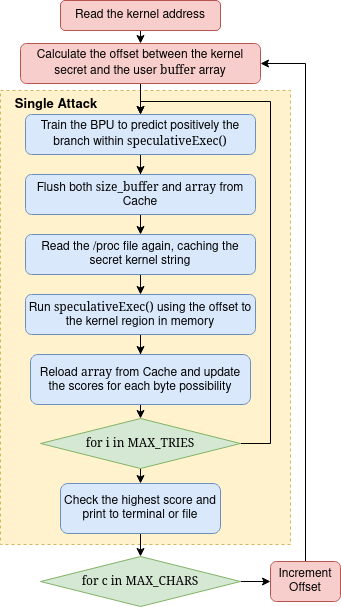
\includegraphics[width=0.4\textwidth]{figures/spectreAttackDiagram.png}
  \caption{Spectre Attack PoC Structure}
  \label{fig:spectreFlowchart}
\end{figure}

All of the developed code can be found in the following git repository on Github (\href{https://github.com/jorge-pais/SSR\_HardwareSecurity}{https://github.com/jorge-pais/SSR\_HardwareSecurity}). This code was developed and tested using a Sony Vaio netbook running an Intel i3-380M processor, which is based on the Westmere architecture from 2010. The operating system utilized was Ubuntu 16.04 running a kernel from 2016 without any mitigations against these microarchitectural exploits in place.



\section{Mitigation}
As soon as these vulnerabilities were found, fix attempts and mitigation techniques were also  deployed. In this section, we describe some possible solutions, mainly as software workarounds, that avoid the need for new hardware. All of the following options presented are available as either a microcode update for each CPU, or Kernel Patches for most Operating Systems.
\subsubsection{Preventing Speculative Execution}
As these attacks are hardware-based, and require speculative execution (SE), the most trivial approach to solve this problem would be to completely disable SE from the CPU. This would, of course, drastically reduce the CPU efficiency and is, therefore, an unfeasible solution.
\subsubsection{KPTI - For Meltdown}
Meltdown attacks break the isolation between kernel and user space. For that, they need to know the memory addresses of the kernel. To make it harder, the OS can randomly set the kernel memory, using KALSR (kernel address space layout randomization) \cite{meltdownPaper}. Still, this does not prevent attacks since the user can still discover the randomized address.
\begin{figure}[h]
  \centering
  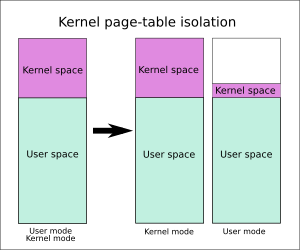
\includegraphics[width=0.36\textwidth]{figures/kpti.png}
  \caption{Kernel Page Table Isolation}
  \label{fig:Kernel Page Table Isolation}
\end{figure}
To further enhance security, operating systems must ensure that user-level programs can never access kernel memory. To do that, Linux deployed KPTI (kernel page table isolation), which consists in creating two-page tables (that map virtual to physical memory), one for kernel-level usage, where all addresses can be accessed, and other for user-level programs, that only map the kernel memory positions needed for the application, thus decreasing the attack surface \cite{databricksMitigations}. Other operating systems, like Windows or Mac OS, also deployed similar solutions.

\subsubsection{Retpoline - For Spectre}
In order to mitigate the effects of Branch Target Injection (i.e. Spectre V2), Google's Project Zero team developed Retpoline \cite{retpolineIntel}. This mitigation strategy works by redirecting indirect branches to a different target address, in a way that does not cause vulnerable speculative execution. 


\section{Conclusion}
This paper briefly presented two system vulnerabilities, Spectre and Meltdown, that take advantage of faulty CPU design to gain access to unauthorized information. A summary of the fundamental theoretical concepts involved is provided, as well as how a simple implementation, based on seed labs, can be made. The work that was developed also gave the students an insight into the relevance of side-channel attacks, and how the simplest of oversights in the design of hardware can expose fatal security flaws.

In the final part, a demonstration of a simple proof-of-concept was developed for a Spectre-styled attack, which could be in theory used to leak information from faulty Linux kernel modules. It is relevant to point out that when the Linux kernel of the testbench PC was finally updated, the exploit no longer worked. 

Concluding, it can be said that all the objectives set out initially for the project were met and that the development of the SEED Labs along with the main contribution helped deepen the knowledge of the students in not only these particular vulnerabilities and their nuances, but also on side-channel attacks in general. 


% trigger a \newpage just before the given reference
% number - used to balance the columns on the last page
% adjust value as needed - may need to be readjusted if
% the document is modified later
%\IEEEtriggeratref{8}
% The "triggered" command can be changed if desired:
%\IEEEtriggercmd{\enlargethispage{-5in}}

% references section

% can use a bibliography generated by BibTeX as a .bbl file
% BibTeX documentation can be easily obtained at:
% http://mirror.ctan.org/biblio/bibtex/contrib/doc/
% The IEEEtran BibTeX style support page is at:
% http://www.michaelshell.org/tex/ieeetran/bibtex/
%\bibliographystyle{IEEEtran}
% argument is your BibTeX string definitions and bibliography database(s)
%\bibliography{IEEEabrv,../bib/paper}
%
% <OR> manually copy in the resultant .bbl file
% set second argument of \begin to the number of references
% (used to reserve space for the reference number labels box)

\bibliography{sample}


% that's all folks
\end{document}
 